% Created by tikzDevice version 0.12 on 2019-04-06 18:44:05
% !TEX encoding = UTF-8 Unicode
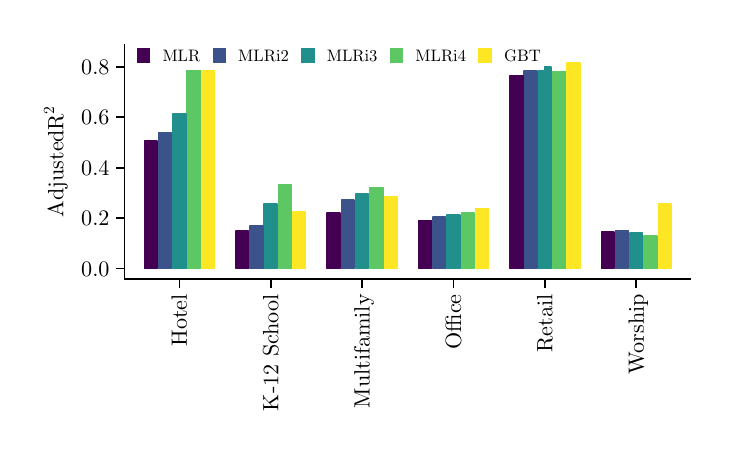
\begin{tikzpicture}[x=1pt,y=1pt]
\definecolor{fillColor}{RGB}{255,255,255}
\path[use as bounding box,fill=fillColor,fill opacity=0.00] (0,0) rectangle (245.72,144.54);
\begin{scope}
\path[clip] (  0.00,  0.00) rectangle (245.72,144.54);
\definecolor{drawColor}{RGB}{255,255,255}
\definecolor{fillColor}{RGB}{255,255,255}

\path[draw=drawColor,line width= 0.6pt,line join=round,line cap=round,fill=fillColor] (  0.00,  0.00) rectangle (245.72,144.54);
\end{scope}
\begin{scope}
\path[clip] ( 34.98, 53.61) rectangle (239.72,138.54);
\definecolor{fillColor}{RGB}{255,255,255}

\path[fill=fillColor] ( 34.98, 53.61) rectangle (239.72,138.54);
\definecolor{drawColor}{RGB}{253,231,37}
\definecolor{fillColor}{RGB}{253,231,37}

\path[draw=drawColor,line width= 0.6pt,line join=round,fill=fillColor] ( 62.79, 57.47) rectangle ( 67.41,134.68);
\definecolor{drawColor}{RGB}{93,200,99}
\definecolor{fillColor}{RGB}{93,200,99}

\path[draw=drawColor,line width= 0.6pt,line join=round,fill=fillColor] ( 57.64, 57.47) rectangle ( 62.26,131.67);
\definecolor{drawColor}{RGB}{33,144,140}
\definecolor{fillColor}{RGB}{33,144,140}

\path[draw=drawColor,line width= 0.6pt,line join=round,fill=fillColor] ( 52.48, 57.47) rectangle ( 57.11,113.35);
\definecolor{drawColor}{RGB}{59,82,139}
\definecolor{fillColor}{RGB}{59,82,139}

\path[draw=drawColor,line width= 0.6pt,line join=round,fill=fillColor] ( 47.33, 57.47) rectangle ( 51.96,106.42);
\definecolor{drawColor}{RGB}{68,1,84}
\definecolor{fillColor}{RGB}{68,1,84}

\path[draw=drawColor,line width= 0.6pt,line join=round,fill=fillColor] ( 42.18, 57.47) rectangle ( 46.80,103.69);
\definecolor{drawColor}{RGB}{253,231,37}
\definecolor{fillColor}{RGB}{253,231,37}

\path[draw=drawColor,line width= 0.6pt,line join=round,fill=fillColor] ( 95.81, 57.47) rectangle (100.43, 77.89);
\definecolor{drawColor}{RGB}{93,200,99}
\definecolor{fillColor}{RGB}{93,200,99}

\path[draw=drawColor,line width= 0.6pt,line join=round,fill=fillColor] ( 90.66, 57.47) rectangle ( 95.28, 87.64);
\definecolor{drawColor}{RGB}{33,144,140}
\definecolor{fillColor}{RGB}{33,144,140}

\path[draw=drawColor,line width= 0.6pt,line join=round,fill=fillColor] ( 85.51, 57.47) rectangle ( 90.13, 80.81);
\definecolor{drawColor}{RGB}{59,82,139}
\definecolor{fillColor}{RGB}{59,82,139}

\path[draw=drawColor,line width= 0.6pt,line join=round,fill=fillColor] ( 80.35, 57.47) rectangle ( 84.98, 72.79);
\definecolor{drawColor}{RGB}{68,1,84}
\definecolor{fillColor}{RGB}{68,1,84}

\path[draw=drawColor,line width= 0.6pt,line join=round,fill=fillColor] ( 75.20, 57.47) rectangle ( 79.83, 71.15);
\definecolor{drawColor}{RGB}{253,231,37}
\definecolor{fillColor}{RGB}{253,231,37}

\path[draw=drawColor,line width= 0.6pt,line join=round,fill=fillColor] (128.83, 57.47) rectangle (133.45, 83.54);
\definecolor{drawColor}{RGB}{93,200,99}
\definecolor{fillColor}{RGB}{93,200,99}

\path[draw=drawColor,line width= 0.6pt,line join=round,fill=fillColor] (123.68, 57.47) rectangle (128.30, 86.73);
\definecolor{drawColor}{RGB}{33,144,140}
\definecolor{fillColor}{RGB}{33,144,140}

\path[draw=drawColor,line width= 0.6pt,line join=round,fill=fillColor] (118.53, 57.47) rectangle (123.15, 84.55);
\definecolor{drawColor}{RGB}{59,82,139}
\definecolor{fillColor}{RGB}{59,82,139}

\path[draw=drawColor,line width= 0.6pt,line join=round,fill=fillColor] (113.38, 57.47) rectangle (118.00, 82.27);
\definecolor{drawColor}{RGB}{68,1,84}
\definecolor{fillColor}{RGB}{68,1,84}

\path[draw=drawColor,line width= 0.6pt,line join=round,fill=fillColor] (108.23, 57.47) rectangle (112.85, 77.53);
\definecolor{drawColor}{RGB}{253,231,37}
\definecolor{fillColor}{RGB}{253,231,37}

\path[draw=drawColor,line width= 0.6pt,line join=round,fill=fillColor] (161.85, 57.47) rectangle (166.48, 79.17);
\definecolor{drawColor}{RGB}{93,200,99}
\definecolor{fillColor}{RGB}{93,200,99}

\path[draw=drawColor,line width= 0.6pt,line join=round,fill=fillColor] (156.70, 57.47) rectangle (161.32, 77.53);
\definecolor{drawColor}{RGB}{33,144,140}
\definecolor{fillColor}{RGB}{33,144,140}

\path[draw=drawColor,line width= 0.6pt,line join=round,fill=fillColor] (151.55, 57.47) rectangle (156.17, 76.80);
\definecolor{drawColor}{RGB}{59,82,139}
\definecolor{fillColor}{RGB}{59,82,139}

\path[draw=drawColor,line width= 0.6pt,line join=round,fill=fillColor] (146.40, 57.47) rectangle (151.02, 76.07);
\definecolor{drawColor}{RGB}{68,1,84}
\definecolor{fillColor}{RGB}{68,1,84}

\path[draw=drawColor,line width= 0.6pt,line join=round,fill=fillColor] (141.25, 57.47) rectangle (145.87, 74.88);
\definecolor{drawColor}{RGB}{253,231,37}
\definecolor{fillColor}{RGB}{253,231,37}

\path[draw=drawColor,line width= 0.6pt,line join=round,fill=fillColor] (194.87, 57.47) rectangle (199.50,131.95);
\definecolor{drawColor}{RGB}{93,200,99}
\definecolor{fillColor}{RGB}{93,200,99}

\path[draw=drawColor,line width= 0.6pt,line join=round,fill=fillColor] (189.72, 57.47) rectangle (194.35,128.75);
\definecolor{drawColor}{RGB}{33,144,140}
\definecolor{fillColor}{RGB}{33,144,140}

\path[draw=drawColor,line width= 0.6pt,line join=round,fill=fillColor] (184.57, 57.47) rectangle (189.19,130.30);
\definecolor{drawColor}{RGB}{59,82,139}
\definecolor{fillColor}{RGB}{59,82,139}

\path[draw=drawColor,line width= 0.6pt,line join=round,fill=fillColor] (179.42, 57.47) rectangle (184.04,128.85);
\definecolor{drawColor}{RGB}{68,1,84}
\definecolor{fillColor}{RGB}{68,1,84}

\path[draw=drawColor,line width= 0.6pt,line join=round,fill=fillColor] (174.27, 57.47) rectangle (178.89,127.30);
\definecolor{drawColor}{RGB}{253,231,37}
\definecolor{fillColor}{RGB}{253,231,37}

\path[draw=drawColor,line width= 0.6pt,line join=round,fill=fillColor] (227.90, 57.47) rectangle (232.52, 80.81);
\definecolor{drawColor}{RGB}{93,200,99}
\definecolor{fillColor}{RGB}{93,200,99}

\path[draw=drawColor,line width= 0.6pt,line join=round,fill=fillColor] (222.74, 57.47) rectangle (227.37, 69.32);
\definecolor{drawColor}{RGB}{33,144,140}
\definecolor{fillColor}{RGB}{33,144,140}

\path[draw=drawColor,line width= 0.6pt,line join=round,fill=fillColor] (217.59, 57.47) rectangle (222.22, 70.42);
\definecolor{drawColor}{RGB}{59,82,139}
\definecolor{fillColor}{RGB}{59,82,139}

\path[draw=drawColor,line width= 0.6pt,line join=round,fill=fillColor] (212.44, 57.47) rectangle (217.07, 71.24);
\definecolor{drawColor}{RGB}{68,1,84}
\definecolor{fillColor}{RGB}{68,1,84}

\path[draw=drawColor,line width= 0.6pt,line join=round,fill=fillColor] (207.29, 57.47) rectangle (211.91, 70.69);
\end{scope}
\begin{scope}
\path[clip] (  0.00,  0.00) rectangle (245.72,144.54);
\definecolor{drawColor}{RGB}{0,0,0}

\path[draw=drawColor,line width= 0.6pt,line join=round] ( 34.98, 53.61) --
	( 34.98,138.54);
\end{scope}
\begin{scope}
\path[clip] (  0.00,  0.00) rectangle (245.72,144.54);
\definecolor{drawColor}{RGB}{0,0,0}

\node[text=drawColor,anchor=base east,inner sep=0pt, outer sep=0pt, scale=  0.80] at ( 29.58, 54.72) {0.0};

\node[text=drawColor,anchor=base east,inner sep=0pt, outer sep=0pt, scale=  0.80] at ( 29.58, 72.95) {0.2};

\node[text=drawColor,anchor=base east,inner sep=0pt, outer sep=0pt, scale=  0.80] at ( 29.58, 91.18) {0.4};

\node[text=drawColor,anchor=base east,inner sep=0pt, outer sep=0pt, scale=  0.80] at ( 29.58,109.41) {0.6};

\node[text=drawColor,anchor=base east,inner sep=0pt, outer sep=0pt, scale=  0.80] at ( 29.58,127.64) {0.8};
\end{scope}
\begin{scope}
\path[clip] (  0.00,  0.00) rectangle (245.72,144.54);
\definecolor{drawColor}{RGB}{0,0,0}

\path[draw=drawColor,line width= 0.6pt,line join=round] ( 31.98, 57.47) --
	( 34.98, 57.47);

\path[draw=drawColor,line width= 0.6pt,line join=round] ( 31.98, 75.70) --
	( 34.98, 75.70);

\path[draw=drawColor,line width= 0.6pt,line join=round] ( 31.98, 93.93) --
	( 34.98, 93.93);

\path[draw=drawColor,line width= 0.6pt,line join=round] ( 31.98,112.16) --
	( 34.98,112.16);

\path[draw=drawColor,line width= 0.6pt,line join=round] ( 31.98,130.40) --
	( 34.98,130.40);
\end{scope}
\begin{scope}
\path[clip] (  0.00,  0.00) rectangle (245.72,144.54);
\definecolor{drawColor}{RGB}{0,0,0}

\path[draw=drawColor,line width= 0.6pt,line join=round] ( 34.98, 53.61) --
	(239.72, 53.61);
\end{scope}
\begin{scope}
\path[clip] (  0.00,  0.00) rectangle (245.72,144.54);
\definecolor{drawColor}{RGB}{0,0,0}

\path[draw=drawColor,line width= 0.6pt,line join=round] ( 54.80, 50.61) --
	( 54.80, 53.61);

\path[draw=drawColor,line width= 0.6pt,line join=round] ( 87.82, 50.61) --
	( 87.82, 53.61);

\path[draw=drawColor,line width= 0.6pt,line join=round] (120.84, 50.61) --
	(120.84, 53.61);

\path[draw=drawColor,line width= 0.6pt,line join=round] (153.86, 50.61) --
	(153.86, 53.61);

\path[draw=drawColor,line width= 0.6pt,line join=round] (186.88, 50.61) --
	(186.88, 53.61);

\path[draw=drawColor,line width= 0.6pt,line join=round] (219.90, 50.61) --
	(219.90, 53.61);
\end{scope}
\begin{scope}
\path[clip] (  0.00,  0.00) rectangle (245.72,144.54);
\definecolor{drawColor}{RGB}{0,0,0}

\node[text=drawColor,rotate= 90.00,anchor=base east,inner sep=0pt, outer sep=0pt, scale=  0.80] at ( 57.55, 48.21) {Hotel};

\node[text=drawColor,rotate= 90.00,anchor=base east,inner sep=0pt, outer sep=0pt, scale=  0.80] at ( 90.57, 48.21) {K-12 School};

\node[text=drawColor,rotate= 90.00,anchor=base east,inner sep=0pt, outer sep=0pt, scale=  0.80] at (123.59, 48.21) {Multifamily};

\node[text=drawColor,rotate= 90.00,anchor=base east,inner sep=0pt, outer sep=0pt, scale=  0.80] at (156.62, 48.21) {Office};

\node[text=drawColor,rotate= 90.00,anchor=base east,inner sep=0pt, outer sep=0pt, scale=  0.80] at (189.64, 48.21) {Retail};

\node[text=drawColor,rotate= 90.00,anchor=base east,inner sep=0pt, outer sep=0pt, scale=  0.80] at (222.66, 48.21) {Worship};
\end{scope}
\begin{scope}
\path[clip] (  0.00,  0.00) rectangle (245.72,144.54);
\definecolor{drawColor}{RGB}{0,0,0}

\node[text=drawColor,rotate= 90.00,anchor=base west,inner sep=0pt, outer sep=0pt, scale=  0.80] at ( 12.86, 76.05) {Adjusted };

\node[text=drawColor,rotate= 90.00,anchor=base west,inner sep=0pt, outer sep=0pt, scale=  0.80] at ( 12.86,107.42) {R};

\node[text=drawColor,rotate= 90.00,anchor=base west,inner sep=0pt, outer sep=0pt, scale=  0.56] at (  9.59,113.31) {2};
\end{scope}
\begin{scope}
\path[clip] (  0.00,  0.00) rectangle (245.72,144.54);
\definecolor{fillColor}{RGB}{255,255,255}

\path[fill=fillColor] ( 36.03,129.09) rectangle (186.42,138.54);
\end{scope}
\begin{scope}
\path[clip] (  0.00,  0.00) rectangle (245.72,144.54);
\definecolor{drawColor}{RGB}{68,1,84}
\definecolor{fillColor}{RGB}{68,1,84}

\path[draw=drawColor,line width= 0.6pt,line cap=round,fill=fillColor] ( 39.74,132.17) rectangle ( 44.01,136.83);
\end{scope}
\begin{scope}
\path[clip] (  0.00,  0.00) rectangle (245.72,144.54);
\definecolor{drawColor}{RGB}{59,82,139}
\definecolor{fillColor}{RGB}{59,82,139}

\path[draw=drawColor,line width= 0.6pt,line cap=round,fill=fillColor] ( 67.10,132.17) rectangle ( 71.36,136.83);
\end{scope}
\begin{scope}
\path[clip] (  0.00,  0.00) rectangle (245.72,144.54);
\definecolor{drawColor}{RGB}{33,144,140}
\definecolor{fillColor}{RGB}{33,144,140}

\path[draw=drawColor,line width= 0.6pt,line cap=round,fill=fillColor] ( 99.12,132.17) rectangle (103.38,136.83);
\end{scope}
\begin{scope}
\path[clip] (  0.00,  0.00) rectangle (245.72,144.54);
\definecolor{drawColor}{RGB}{93,200,99}
\definecolor{fillColor}{RGB}{93,200,99}

\path[draw=drawColor,line width= 0.6pt,line cap=round,fill=fillColor] (131.13,132.17) rectangle (135.40,136.83);
\end{scope}
\begin{scope}
\path[clip] (  0.00,  0.00) rectangle (245.72,144.54);
\definecolor{drawColor}{RGB}{253,231,37}
\definecolor{fillColor}{RGB}{253,231,37}

\path[draw=drawColor,line width= 0.6pt,line cap=round,fill=fillColor] (163.15,132.17) rectangle (167.42,136.83);
\end{scope}
\begin{scope}
\path[clip] (  0.00,  0.00) rectangle (245.72,144.54);
\definecolor{drawColor}{RGB}{0,0,0}

\node[text=drawColor,anchor=base west,inner sep=0pt, outer sep=0pt, scale=  0.60] at ( 48.72,132.44) {MLR};
\end{scope}
\begin{scope}
\path[clip] (  0.00,  0.00) rectangle (245.72,144.54);
\definecolor{drawColor}{RGB}{0,0,0}

\node[text=drawColor,anchor=base west,inner sep=0pt, outer sep=0pt, scale=  0.60] at ( 76.07,132.44) {MLRi2};
\end{scope}
\begin{scope}
\path[clip] (  0.00,  0.00) rectangle (245.72,144.54);
\definecolor{drawColor}{RGB}{0,0,0}

\node[text=drawColor,anchor=base west,inner sep=0pt, outer sep=0pt, scale=  0.60] at (108.09,132.44) {MLRi3};
\end{scope}
\begin{scope}
\path[clip] (  0.00,  0.00) rectangle (245.72,144.54);
\definecolor{drawColor}{RGB}{0,0,0}

\node[text=drawColor,anchor=base west,inner sep=0pt, outer sep=0pt, scale=  0.60] at (140.11,132.44) {MLRi4};
\end{scope}
\begin{scope}
\path[clip] (  0.00,  0.00) rectangle (245.72,144.54);
\definecolor{drawColor}{RGB}{0,0,0}

\node[text=drawColor,anchor=base west,inner sep=0pt, outer sep=0pt, scale=  0.60] at (172.13,132.44) {GBT};
\end{scope}
\end{tikzpicture}
